\documentclass[a4paper,12pt]{report}

\usepackage[english]{babel}
\usepackage[utf8]{inputenc}
\usepackage{indentfirst,setspace,subcaption}
\usepackage{amsmath,amssymb,graphicx,xcolor,url}
\usepackage{fancyhdr,tocbasic,titlesec,listings}
\usepackage[a4paper,margin=24mm]{geometry}
\usepackage[skip=10pt plus1pt, indent=20pt]{parskip}
\usepackage[colorlinks=true,allcolors=blue,urlcolor=magenta]{hyperref}

\renewcommand{\thesection}{\arabic{section}}

% Header and footer styling
\pagestyle{fancy}
\setlength{\headheight}{15pt}
\fancyhf{}
\fancyhead[R]{\nouppercase\rightmark\hfill~Lab report}
\fancyfoot[C]{\hfill\thepage\hfill}

% TOC styling
\DeclareTOCStyleEntry[
  indent=12pt,
  level=1
]{largetocline}{section}

% Title page data
\title{Implementing Hash Table from scratch}
\author{Ngo Nguyen The Khoa -- 23127065 -- 23CLC09}
\date{August 6, 2024}

\begin{document}

% Title page and TOC
\thispagestyle{empty}
\begin{titlepage}
	\begin{center}
		\makeatletter
		\newcommand{\HRule}{\rule{\linewidth}{0.4mm}}

		\textsc{\LARGE Vietnam National University,\\Ho Chi Minh City}\\[1.5cm]
		\textsc{\Large University of Science}\\[0.5cm]
		\textsc{\Large Faculty of Information Technology}\\[1.5cm]

		{\HRule}\\[1cm]
		{\huge \bfseries \@title}\\[0.5cm]
		{\HRule}\\[2cm]

		\textsc{\large CSC10004 -- Data Structures and Algorithms}\\[0.5cm]

		\vfill\vfill\vfill

		{\large \@author}\\[1.5cm]
		{\large \@date}
		\makeatother
	\end{center}
\end{titlepage}
\tableofcontents\thispagestyle{empty}

\pagebreak
\section{How I implemented the requirements}
\begin{flushleft}
  I implemented the requirements as follows:
  \begin{itemize}
    \item The second hash function I have used for \textsl{`Double Hashing'} is\\~\(h_2(k) = 1 + (k \mod (m - 1))\), where \(m\) is the size of the hash table.
    \item With \textsl{`Double Hashing'} and \textsl{`Quadratic Probing'} methods, I have maintained a hash table which its size is a prime number larger than the real size to avoid collisions as much as possible.
    \item I didn't implement rehashing for \textsl{`Double Hashing'} and \textsl{`Quadratic Probing'} because the size of the hash table is fixed, so it could cause `not-found' situation in some cases. (You can find those in the \textsl{`Double Hashing'} and \textsl{`Quadratic Probing'} experiment sections in this report.)
    \item Although there was no rehashing implementation in my source, I tested using rehashing for \textsl{`Double Hashing'} and \textsl{`Quadratic Probing'} methods to solve the collisions.
          \begin{itemize}
            \item \textbf{Rehashing using \textit{`double the size'}:} I have to rehash 8 times, which means the size is a prime number larger than \(3e5\cdot256\) to avoid missing some records.
            \item \textbf{Rehashing using \textit{`prime number sizing'}:} I have to resize the hash table to \(58500011\approx 3e5\cdot195\) to avoid missing some records.
          \end{itemize}
  \end{itemize}
\end{flushleft}

\pagebreak
\section{Result Screenshots}
\pagebreak
\subsection{Double Hashing Operations}
\begin{figure}[!ht]
	\centering
	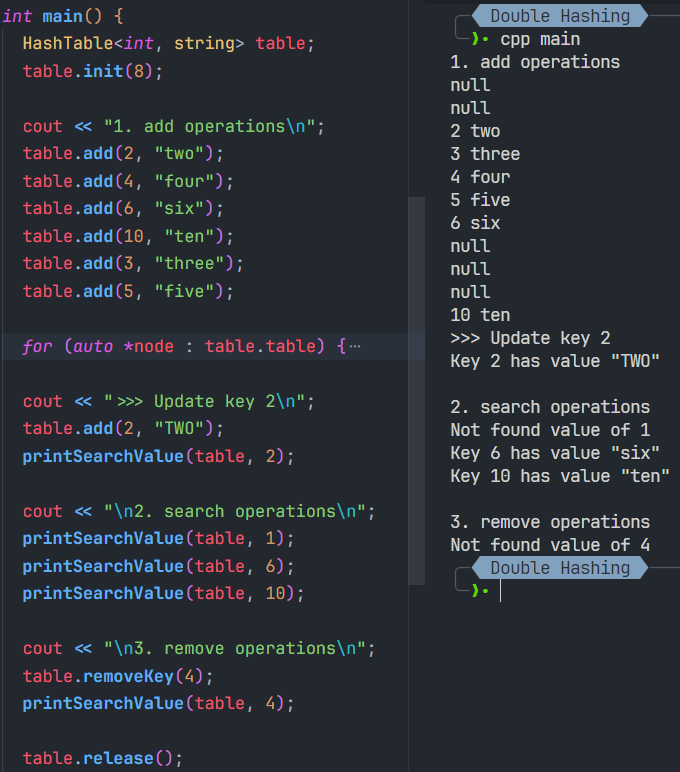
\includegraphics[width=\textwidth]{imgs/Double Hashing/operations.png}
	\caption{Screenshot of Double Hashing operations.}\label{fig:dblhashing-operations}
\end{figure}
\pagebreak
\subsection{Double Hashing Operations}
\begin{figure}[!ht]
	\centering
	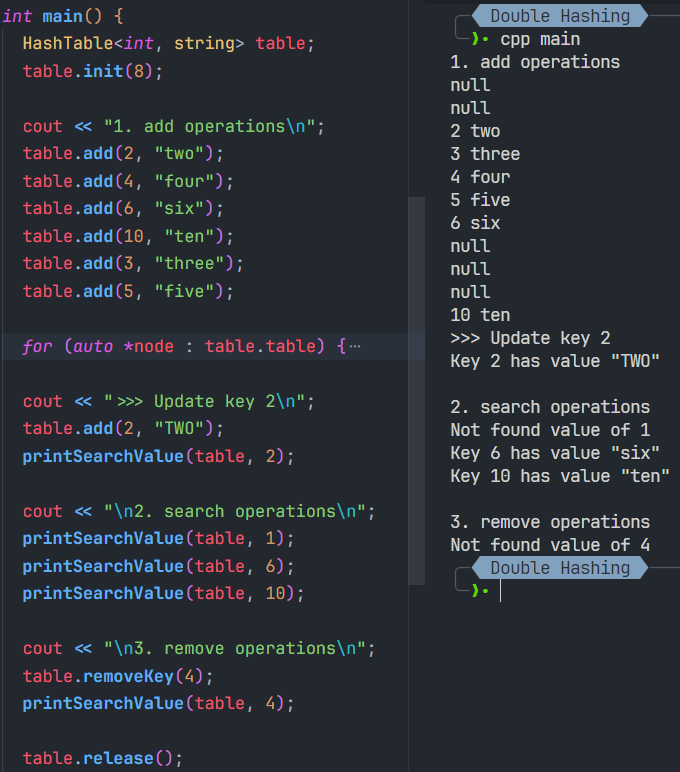
\includegraphics[width=\textwidth]{imgs/Double Hashing/operations.png}
	\caption{Screenshot of Double Hashing operations.}\label{fig:dblhashing-operations}
\end{figure}
\pagebreak
\subsection{Double Hashing Operations}
\begin{figure}[!ht]
	\centering
	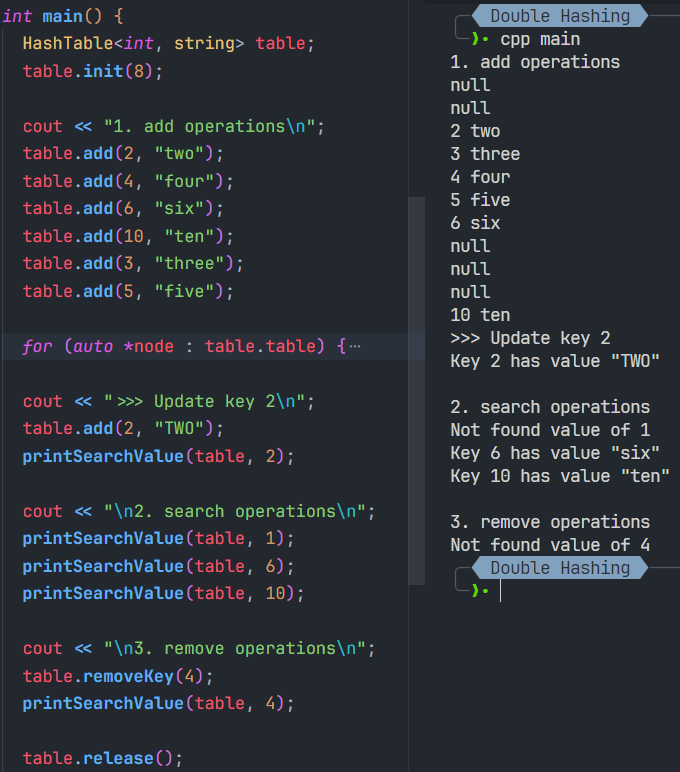
\includegraphics[width=\textwidth]{imgs/Double Hashing/operations.png}
	\caption{Screenshot of Double Hashing operations.}\label{fig:dblhashing-operations}
\end{figure}
\pagebreak
\subsection{Double Hashing Operations}
\begin{figure}[!ht]
	\centering
	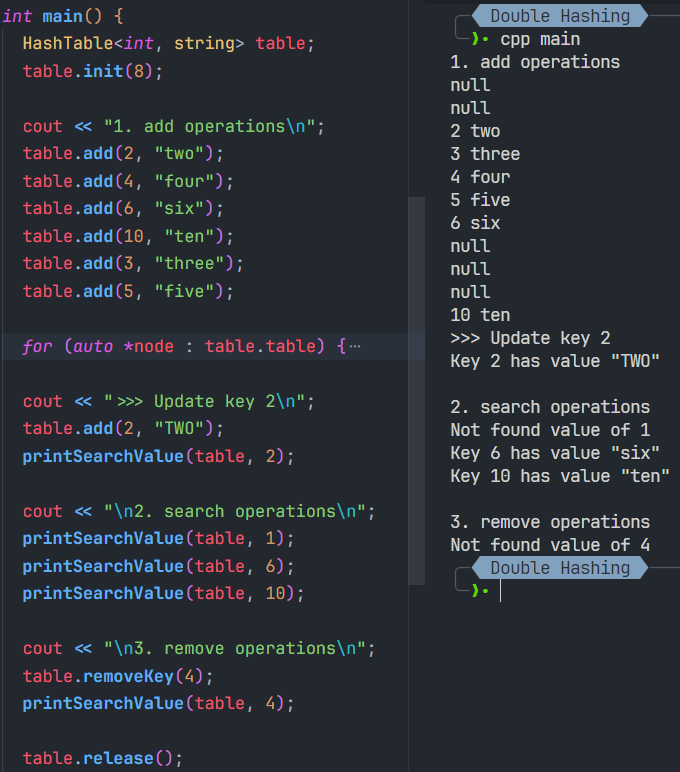
\includegraphics[width=\textwidth]{imgs/Double Hashing/operations.png}
	\caption{Screenshot of Double Hashing operations.}\label{fig:dblhashing-operations}
\end{figure}
\pagebreak
\subsection{Double Hashing Operations}
\begin{figure}[!ht]
	\centering
	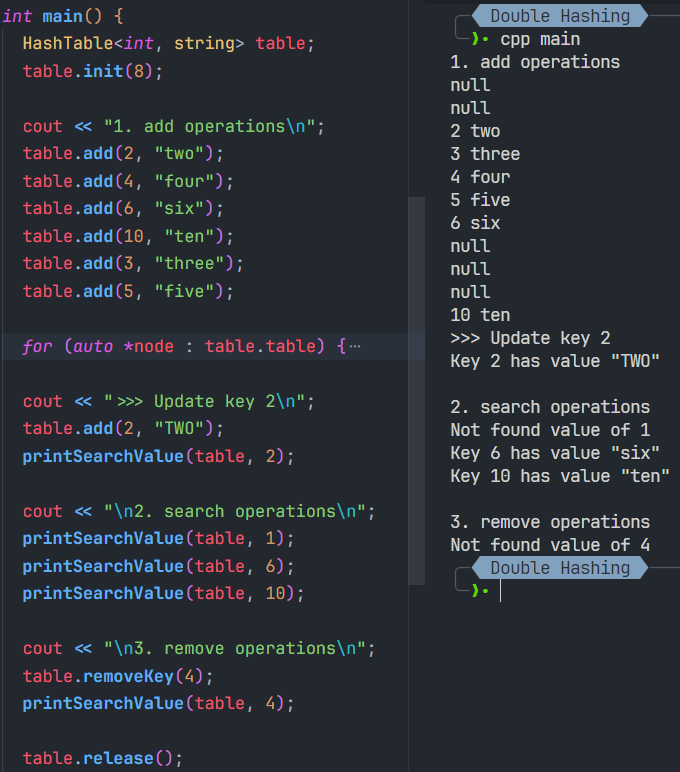
\includegraphics[width=\textwidth]{imgs/Double Hashing/operations.png}
	\caption{Screenshot of Double Hashing operations.}\label{fig:dblhashing-operations}
\end{figure}

\pagebreak
\section{Experiments}
\pagebreak
\subsection{Chaining Linked List and Linear Searching Algorithm}
\begin{itemize}
	\item \textbf{Theoretical Time Complexity:}
	      \begin{itemize}
		      \item The time complexity of searching using Chaining Linked List is \(O(n)\).
		      \item The time complexity of searching using Linear Searching Algorithm is \(O(n)\).
	      \end{itemize}
	\item \textbf{Actual execution time:}
	      \begin{itemize}
		      \item Searching using Chaining Linked List is faster than using Linear Searching Algorithm in most cases (except there are too many collisions).
	      \end{itemize}
	\item \textbf{Case Screenshots:}
	      \begin{figure}[!ht]
		      \centering
		      \begin{subfigure}{0.45\textwidth}
			      \centering
			      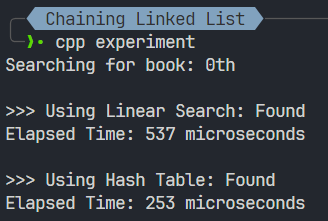
\includegraphics[width=\textwidth]{imgs/Chaining Linked List/beg.png}
			      \caption{When the key is at the begining of Hash Table}\label{fig:chainingll-beg-metric}
		      \end{subfigure}
		      \hfill
		      \begin{subfigure}{0.45\textwidth}
			      \centering
			      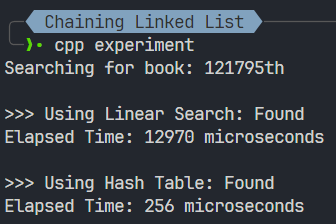
\includegraphics[width=\textwidth]{imgs/Chaining Linked List/mid.png}
			      \caption{When the key is at the middle of Hash Table}\label{fig:chainingll-mid-metric}
		      \end{subfigure}
		      \hfill
		      \begin{subfigure}{0.45\textwidth}
			      \centering
			      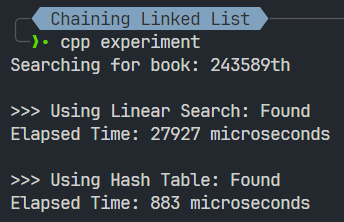
\includegraphics[width=\textwidth]{imgs/Chaining Linked List/end.png}
			      \caption{When the key is at the end of Hash Table}\label{fig:chainingll-end-metric}
		      \end{subfigure}
		      \hfill
		      \begin{subfigure}{0.45\textwidth}
			      \centering
			      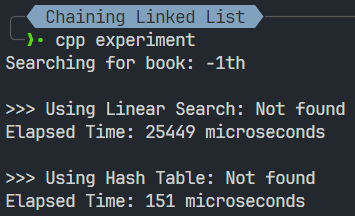
\includegraphics[width=\textwidth]{imgs/Chaining Linked List/not-found.png}
			      \caption{When the key is `not'~in Hash Table}\label{fig:chainingll-notfound-metric}
		      \end{subfigure}

		      \caption{Screenshots of Searching Case with Chaining Linked List.}\label{fig:chainingll-search-metric}
	      \end{figure}
\end{itemize}
\pagebreak
\subsection{Chaining Linked List and Linear Searching Algorithm}
\begin{itemize}
	\item \textbf{Theoretical Time Complexity:}
	      \begin{itemize}
		      \item The time complexity of searching using Chaining Linked List is \(O(n)\).
		      \item The time complexity of searching using Linear Searching Algorithm is \(O(n)\).
	      \end{itemize}
	\item \textbf{Actual execution time:}
	      \begin{itemize}
		      \item Searching using Chaining Linked List is faster than using Linear Searching Algorithm in most cases (except there are too many collisions).
	      \end{itemize}
	\item \textbf{Case Screenshots:}
	      \begin{figure}[!ht]
		      \centering
		      \begin{subfigure}{0.45\textwidth}
			      \centering
			      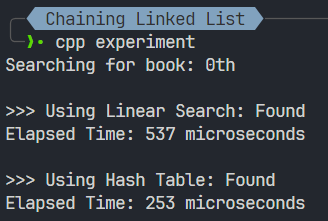
\includegraphics[width=\textwidth]{imgs/Chaining Linked List/beg.png}
			      \caption{When the key is at the begining of Hash Table}\label{fig:chainingll-beg-metric}
		      \end{subfigure}
		      \hfill
		      \begin{subfigure}{0.45\textwidth}
			      \centering
			      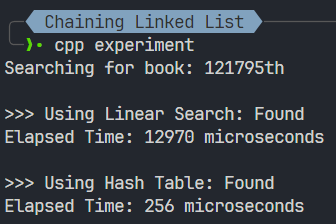
\includegraphics[width=\textwidth]{imgs/Chaining Linked List/mid.png}
			      \caption{When the key is at the middle of Hash Table}\label{fig:chainingll-mid-metric}
		      \end{subfigure}
		      \hfill
		      \begin{subfigure}{0.45\textwidth}
			      \centering
			      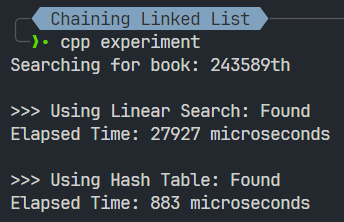
\includegraphics[width=\textwidth]{imgs/Chaining Linked List/end.png}
			      \caption{When the key is at the end of Hash Table}\label{fig:chainingll-end-metric}
		      \end{subfigure}
		      \hfill
		      \begin{subfigure}{0.45\textwidth}
			      \centering
			      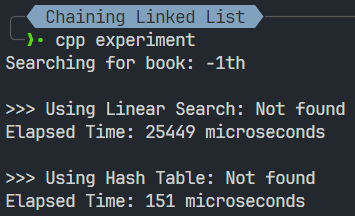
\includegraphics[width=\textwidth]{imgs/Chaining Linked List/not-found.png}
			      \caption{When the key is `not'~in Hash Table}\label{fig:chainingll-notfound-metric}
		      \end{subfigure}

		      \caption{Screenshots of Searching Case with Chaining Linked List.}\label{fig:chainingll-search-metric}
	      \end{figure}
\end{itemize}
\pagebreak
\subsection{Chaining Linked List and Linear Searching Algorithm}
\begin{itemize}
	\item \textbf{Theoretical Time Complexity:}
	      \begin{itemize}
		      \item The time complexity of searching using Chaining Linked List is \(O(n)\).
		      \item The time complexity of searching using Linear Searching Algorithm is \(O(n)\).
	      \end{itemize}
	\item \textbf{Actual execution time:}
	      \begin{itemize}
		      \item Searching using Chaining Linked List is faster than using Linear Searching Algorithm in most cases (except there are too many collisions).
	      \end{itemize}
	\item \textbf{Case Screenshots:}
	      \begin{figure}[!ht]
		      \centering
		      \begin{subfigure}{0.45\textwidth}
			      \centering
			      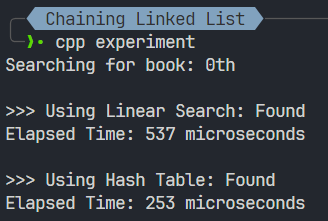
\includegraphics[width=\textwidth]{imgs/Chaining Linked List/beg.png}
			      \caption{When the key is at the begining of Hash Table}\label{fig:chainingll-beg-metric}
		      \end{subfigure}
		      \hfill
		      \begin{subfigure}{0.45\textwidth}
			      \centering
			      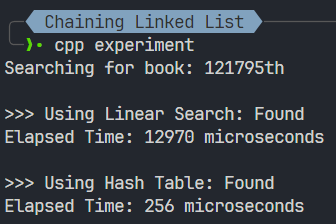
\includegraphics[width=\textwidth]{imgs/Chaining Linked List/mid.png}
			      \caption{When the key is at the middle of Hash Table}\label{fig:chainingll-mid-metric}
		      \end{subfigure}
		      \hfill
		      \begin{subfigure}{0.45\textwidth}
			      \centering
			      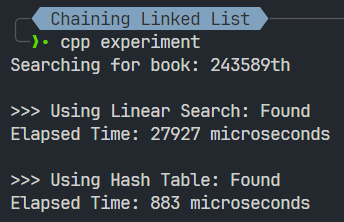
\includegraphics[width=\textwidth]{imgs/Chaining Linked List/end.png}
			      \caption{When the key is at the end of Hash Table}\label{fig:chainingll-end-metric}
		      \end{subfigure}
		      \hfill
		      \begin{subfigure}{0.45\textwidth}
			      \centering
			      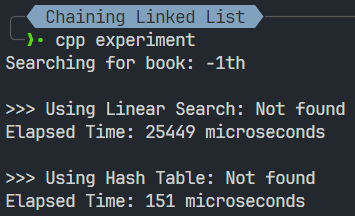
\includegraphics[width=\textwidth]{imgs/Chaining Linked List/not-found.png}
			      \caption{When the key is `not'~in Hash Table}\label{fig:chainingll-notfound-metric}
		      \end{subfigure}

		      \caption{Screenshots of Searching Case with Chaining Linked List.}\label{fig:chainingll-search-metric}
	      \end{figure}
\end{itemize}
\pagebreak
\subsection{Chaining Linked List and Linear Searching Algorithm}
\begin{itemize}
	\item \textbf{Theoretical Time Complexity:}
	      \begin{itemize}
		      \item The time complexity of searching using Chaining Linked List is \(O(n)\).
		      \item The time complexity of searching using Linear Searching Algorithm is \(O(n)\).
	      \end{itemize}
	\item \textbf{Actual execution time:}
	      \begin{itemize}
		      \item Searching using Chaining Linked List is faster than using Linear Searching Algorithm in most cases (except there are too many collisions).
	      \end{itemize}
	\item \textbf{Case Screenshots:}
	      \begin{figure}[!ht]
		      \centering
		      \begin{subfigure}{0.45\textwidth}
			      \centering
			      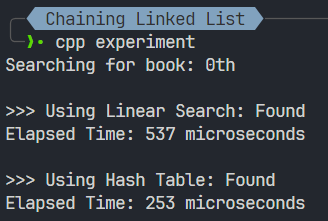
\includegraphics[width=\textwidth]{imgs/Chaining Linked List/beg.png}
			      \caption{When the key is at the begining of Hash Table}\label{fig:chainingll-beg-metric}
		      \end{subfigure}
		      \hfill
		      \begin{subfigure}{0.45\textwidth}
			      \centering
			      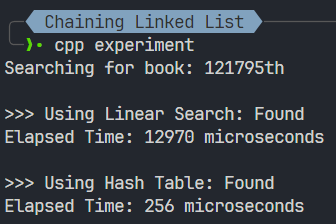
\includegraphics[width=\textwidth]{imgs/Chaining Linked List/mid.png}
			      \caption{When the key is at the middle of Hash Table}\label{fig:chainingll-mid-metric}
		      \end{subfigure}
		      \hfill
		      \begin{subfigure}{0.45\textwidth}
			      \centering
			      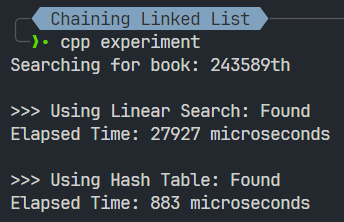
\includegraphics[width=\textwidth]{imgs/Chaining Linked List/end.png}
			      \caption{When the key is at the end of Hash Table}\label{fig:chainingll-end-metric}
		      \end{subfigure}
		      \hfill
		      \begin{subfigure}{0.45\textwidth}
			      \centering
			      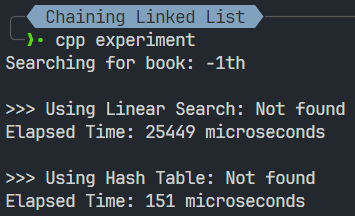
\includegraphics[width=\textwidth]{imgs/Chaining Linked List/not-found.png}
			      \caption{When the key is `not'~in Hash Table}\label{fig:chainingll-notfound-metric}
		      \end{subfigure}

		      \caption{Screenshots of Searching Case with Chaining Linked List.}\label{fig:chainingll-search-metric}
	      \end{figure}
\end{itemize}
\pagebreak
\subsection{Chaining Linked List and Linear Searching Algorithm}
\begin{itemize}
	\item \textbf{Theoretical Time Complexity:}
	      \begin{itemize}
		      \item The time complexity of searching using Chaining Linked List is \(O(n)\).
		      \item The time complexity of searching using Linear Searching Algorithm is \(O(n)\).
	      \end{itemize}
	\item \textbf{Actual execution time:}
	      \begin{itemize}
		      \item Searching using Chaining Linked List is faster than using Linear Searching Algorithm in most cases (except there are too many collisions).
	      \end{itemize}
	\item \textbf{Case Screenshots:}
	      \begin{figure}[!ht]
		      \centering
		      \begin{subfigure}{0.45\textwidth}
			      \centering
			      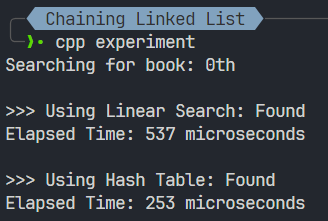
\includegraphics[width=\textwidth]{imgs/Chaining Linked List/beg.png}
			      \caption{When the key is at the begining of Hash Table}\label{fig:chainingll-beg-metric}
		      \end{subfigure}
		      \hfill
		      \begin{subfigure}{0.45\textwidth}
			      \centering
			      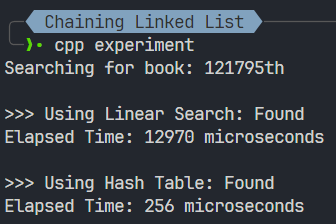
\includegraphics[width=\textwidth]{imgs/Chaining Linked List/mid.png}
			      \caption{When the key is at the middle of Hash Table}\label{fig:chainingll-mid-metric}
		      \end{subfigure}
		      \hfill
		      \begin{subfigure}{0.45\textwidth}
			      \centering
			      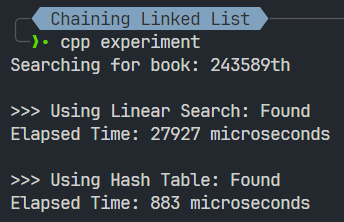
\includegraphics[width=\textwidth]{imgs/Chaining Linked List/end.png}
			      \caption{When the key is at the end of Hash Table}\label{fig:chainingll-end-metric}
		      \end{subfigure}
		      \hfill
		      \begin{subfigure}{0.45\textwidth}
			      \centering
			      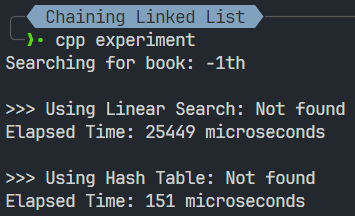
\includegraphics[width=\textwidth]{imgs/Chaining Linked List/not-found.png}
			      \caption{When the key is `not'~in Hash Table}\label{fig:chainingll-notfound-metric}
		      \end{subfigure}

		      \caption{Screenshots of Searching Case with Chaining Linked List.}\label{fig:chainingll-search-metric}
	      \end{figure}
\end{itemize}

\pagebreak
\section{Self-evaluation}
\begin{center}
  \renewcommand{\arraystretch}{1.5}
  \begin{tabular}{|l|p{\dimexpr0.6\linewidth-2\tabcolsep}|c|}
    \hline
    \textbf{No.} & \textbf{Details}           & \textbf{Score} \\ \hline
    1            & Linear Probing             & 100\%          \\ \hline
    2            & Quadratic Probing          & 100\%          \\ \hline
    3            & Chaining using Linked List & 100\%          \\ \hline
    4            & Chaining using AVL Tree    & 100\%          \\ \hline
    5            & Double Hashing             & 100\%          \\ \hline
    6            & Experiments                & 100\%          \\ \hline
    7            & Report                     & 100\%          \\ \hline
  \end{tabular}
\end{center}

\pagebreak
\section{Exercise Feedback}
\subsection{What I have learned from this Exercise}
\begin{flushleft}
  Because almost the things could be done easily, I have learned a few things new from this exercise.
  \begin{itemize}
    \item I have learned how to implement the hash table using different methods of collision handling.
    \item I have learned how to use rehashing to solve the collisions.
    \item I also know how to test the hash table using different test cases.
    \item Have a strong understanding of the hash table and its methods is the big thing I got after finishing this Exercise.
  \end{itemize}
\end{flushleft}
\subsection{What I found challenging}
\begin{flushleft}
  This exercise is quite simple and easy, so I have no difficulties to finish this task.
\end{flushleft}
\subsection{What I have used in this exercise}
\begin{itemize}
  \item I used C++ to implement the data structures and the test cases.
  \item I also used \LaTeX{} to write this report.
\end{itemize}
\end{document}